\chapter{ Констукторский раздел}
\label{cha:design}
    В данном разделе будут рассмотрены схемы алгоритмов, требования к функциональности ПО,
    и опредены способы тестирования.
    
    \section{Разработка алгоритмов}
        Ниже будут представлены схемы алгоритмов сортировки: \begin{enumerate}
            \item алгоритм сортировки пузырьком с флагом (рисунок \ref{schema:sort:bubble});
            \item алгоритм сортировки вставками  (рисунок \ref{schema:sort:insertion});
            \item алгоритм сортировки выбором (рисунок \ref{schema:sort:selection}).
        \end{enumerate}

    \begin{figure}[h!]
        \centering
            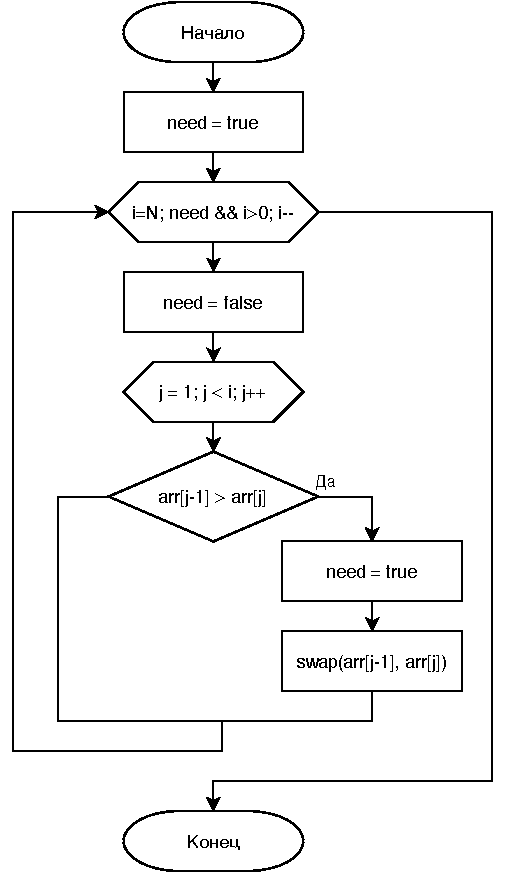
\includegraphics[scale=0.9]{schema_bubble.pdf}
            \caption{Схема алгоритма сортировки пузырьком с флагом}
            \label{schema:sort:bubble}
    \end{figure}

    \begin{figure}[h!]
        \centering
            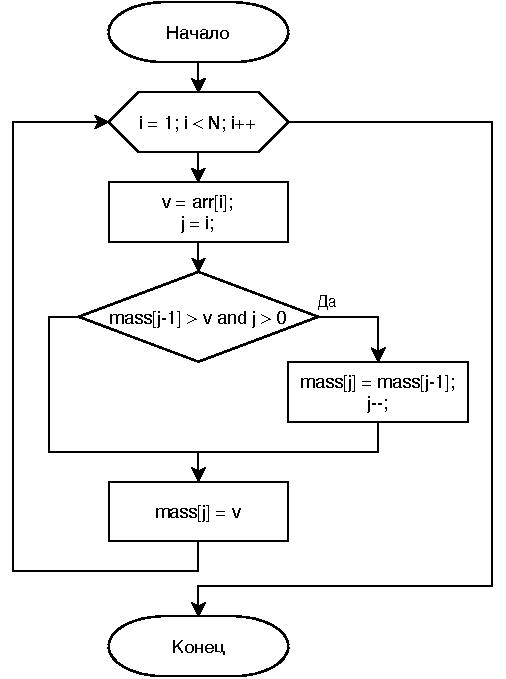
\includegraphics[scale=0.9]{schema_insertion.pdf}
            \caption{Схема алгоритма сортировки вставками}
            \label{schema:sort:insertion}
    \end{figure}

    \begin{figure}[h!]
        \centering
            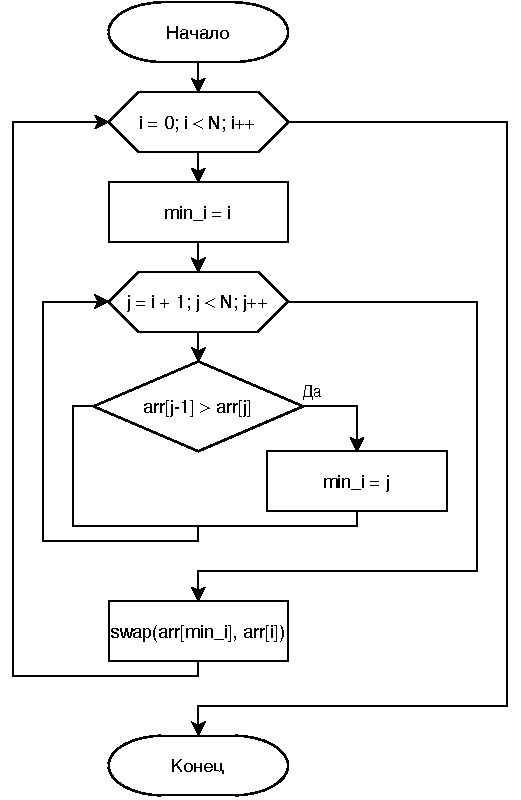
\includegraphics[scale=0.9]{schema_selection.pdf}
            \caption{Схема алгоритма сортировки выбором}
            \label{schema:sort:selection}
    \end{figure}

    \section{Требования к функциональности ПО}
        В данной работе требуется обеспечить следующую минимальную функциональность консольного приложения:
        \begin{enumerate}
            \item предоставить возможность ввода массива, на выходе пользователь должен получить результат сортировки массива, произведенной тремя алгоритмами;
            \item обеспечить вывод замеров времени работы каждого из алгоритмов в худшем, лучшем и произвольном случаях.
        \end{enumerate}

    \section{Тесты}
    Тестирование ПО будет проводиться методом чёрного ящика. Необходимо проверить работу системы 
    на тривиальных случаях: список является пустым или содержит один элемент,
    и несколько нетривальных случаев: список отсортирован по возрастанию / по убыванию, случайный список.

\newpage